\documentclass[10pt,landscape, fleqn]{article}
\usepackage{multicol}
\usepackage{mathtools}
\usepackage{calc}
\usepackage{ifthen}
\usepackage[landscape]{geometry}
\usepackage{hyperref}
\usepackage[calcwidth]{titlesec}
\usepackage{enumitem}

\ifthenelse{\lengthtest { \paperwidth = 11in}}
{ \geometry{top=.5in,left=.5in,right=.5in,bottom=.5in} }
{\ifthenelse{ \lengthtest{ \paperwidth = 297mm}}
	{\geometry{top=1cm,left=1cm,right=1cm,bottom=1cm} }
	{\geometry{top=1cm,left=1cm,right=1cm,bottom=1cm} }
}

% Do not indent equations
\setlength{\mathindent}{0pt}


% Turn off header and footer
\pagestyle{empty}


% Redefine section commands to use less space
%\makeatletter
%\renewcommand{\section}{\@startsection{section}{1}{0mm}% 
%	{-1ex plus -.5ex minus -.2ex}%
%	{0.5ex plus .2ex}%x
%	{\normalfont\large\bfseries}
%	}
\titleformat{\section} {\normalfont\large\bfseries}{\thesection}{1em}{}[{\titlerule[1.5pt]}]
\titlespacing{\section}{0.0em}{.5ex}{.5ex} % {left}{before}{after}[right]
%\renewcommand{\subsection}{\@startsection{subsection}{2}{0mm}%
%	{-1explus -.5ex minus -.2ex}%
%	{0.5ex plus .2ex}%
%	{\normalfont\normalsize\bfseries}}
\titleformat{\subsection}{\normalfont\normalsize\bfseries}{\thesection}{0.5em}{}[\vspace{-1em}\rule{\titlewidth}{0.3pt}]
\titlespacing{\subsection}{0.0em}{0ex}{0ex} % {left}{before}{after}[right]
% \renewcommand{\subsubsection}{\@startsection{subsubsection}{3}{0mm}%
%	{-1ex plus -.5ex minus -.2ex}%
%	{1ex plus .2ex}% 
%	{\normalfont\small\bfseries}}
%\makeatother
\titleformat{\subsubsection} {\normalfont\small\bfseries}{\thesection}{0.5em}{}
\titlespacing{\subsubsection}{0.0em}{0ex}{0ex} % {left}{before}{after}[right]

\setlist[itemize]{leftmargin=*}
\setlist[enumerate]{leftmargin=*}

% Define BibTeX command
\def\BibTeX{{\rm B\kern-.05em{\sc i\kern-.025em b}\kern-.08em
		T\kern-.1667em\lower.7ex\hbox{E}\kern-.125emX}}

% Don't print section numbers
\setcounter{secnumdepth}{0}


\setlength{\parindent}{0pt}
\setlength{\parskip}{2pt plus 0.5ex}


% -----------------------------------------------------------------------

\begin{document}
	\raggedright
	\footnotesize
	
	\begin{center}
		\Large{\textbf{Generalised Linear Modelling Cheat Sheet}} \\
	\end{center}
	\begin{multicols}{3}
		% multicol parameters
		% These lengths are set only within the two main columns
		%\setlength{\columnseprule}{0.25pt}
		\setlength{\premulticols}{1pt}
		\setlength{\postmulticols}{1pt}
		\setlength{\multicolsep}{1pt}
		\setlength{\columnsep}{2pt}
		
		\section{GLMs}
			\subsection{Key Components}
				\begin{enumerate}
					\item A set of response data. $E[Y_i] = \mu_i$
					\item A set of predictors. 
					\item A data distribution $P(Y_i|X_i)$ that is the error component of the model
					\item A \textbf{link} function $g$, $g(\mu_i) = x_i^T\beta = \eta_i$
						  \begin{enumerate}
						  	\item Monotone
						  	\item Continuous
						  	\item Differentiable
						  \end{enumerate}
					\item Independent observation assumption (observations are uncorrelated)
				\end{enumerate}
			\subsection{Common GLMs}
				\begin{enumerate}
					\item Gaussian GLM
					\item Logistic regression binary data
					\item Logistic regression binomial data
					\item Poisson regression
					\item Gamma GLM
					\item Multinomial GLM
				\end{enumerate}
			\subsection{Exponential Families}
				A member of exponential families has a pdf of the form:
				\[ f(y_i|\theta_i, \phi) = exp\left\{\frac{y_i\theta_i-b(\theta_i)}{\phi} + c(y_i, \phi) \right\} \]
				$\theta$ : natural parameter, represents location \par 
				$\phi$: dispersion parameter, represents scale \par
				$E[Y] = \mu = b'(\theta)$ \par 
				$Var[Y] = b''(\theta)\phi = V(\mu)\phi$
			\subsection{Canonical Links}
				It the canonical link is chosen, then $X^TY$ is sufficient for estimation of $\beta$.
				\[ \eta_i = g(\mu_i) = \theta = x_i^T\beta \]
				\begin{tabular}{ | l | l | l | }
					\hline
					Distribution & Link Type & Link Function\\
					\hline
					Normal($\mu_i, \sigma^2$) & identity & $\eta_i = \mu_i$ \\
					Poisson($\mu_i$) & log & $\eta_i = log(\mu_i)$ \\
					Binomial($n, p_i$) & logit & $\eta_i = \log(\frac{p_i}{1-pi}) = log(\frac{\mu_i}{1-\mu_i})$ \\
					Gamma($\alpha, \beta_i$) & reciprocal & $\eta_i = -\frac{1}{\mu_i} = -\frac{\beta_i}{\alpha} $ \\
					\hline
				\end{tabular}
				 \par 
				\begin{tabular}{ | l | l | l | l | }
					\hline
					Family & E[Y] & Var($\mu_i$) & $\phi$ \\
					\hline
					Normal($\mu_i, \sigma^2$) & $\eta_i$ & 1 & $\sigma^2$ \\
					Poisson($\mu_i$) & $exp(\eta_i)$ & $\mu_i$  &  $\eta_i = log(\mu_i)$ \\
					Binomial($n, p_i$) & $n\left(\frac{exp(\eta_i)}{1+exp(\eta_i)}\right)$ & $\frac{\mu_i(n-\mu_i)}{n}$ & 1 \\
					Gamma($\alpha, \beta_i$) & $-\frac{1}{\eta_i}$ & $\mu_i^2$ & $\frac{1}{\alpha} \equiv z $ \\
					\hline
				\end{tabular}
			\subsection{Weighted Least Squares(WLS)}
				High variability $\rightarrow$ low weights. \par
				Regression $\sqrt{w_i}y_i$ on $\sqrt{w_i}x_i$ 
				\[ WSS = \sum_{i=1}^{n}w_i^2(y_i-X_i\hat{\beta})^2 \]
				\[ \hat{\beta}_{WLS} = (X^TWX)^{-1}X^TWY \]
				Adjusted residual: $\sqrt{w_i}\hat{\epsilon_i}$
			\subsection{Iteratively Reweighted Least Squares(IRWLS)}
				$g(y) \approx g(u) + (y-u)g'(u) = \eta + (y - u)\frac{d\eta}{d\mu}$ \par 
				Delta Method: $\widehat{Var[g(y)]} \equiv \left(\frac{d\eta}{d\eta}\right)^2V(Y)$
				\begin{enumerate}
					\item set initial estimate $\hat{\eta}_0$ and $\hat{\mu}_0$
					\item $z_0 = \hat{\eta}_0 + (y-\hat{\mu}_0)\frac{d\eta}{d\mu}|_{\hat{\eta}_0}$
					\item $w_0^{-1} = \left( \frac{d\eta}{d\mu} \right)^2|_{\hat{\eta}_0}V(y)$
					\item Regress $\sqrt{w_0}Z$ on $\sqrt{w_0}X$ and get the new $\hat{\eta}$
					\item Iterate steps 2-4 until convergence
				\end{enumerate}
				$\widehat{Var}(\hat{\beta}) = \phi(X^TWX)^{-1}$
				\subsubsection{An Example: Binomial(n,p)}
					\begin{itemize}
						\item $\eta = log\frac{\mu}{1-\mu}$
						\item $\frac{d\eta}{d\mu} = \frac{1}{\mu(1-\mu)}$
						\item $V(Y) = \mu(1-\mu) = np(1-p)$
						\item $w = n\mu(1-\mu)$
					\end{itemize}
			\subsection{Linear combination of MLEs}
				$c$: vector describing the linear combination of $\beta$'s.
				\[E[c^T\hat{\beta}] = c^T\beta \]
				\[Var[c^T\hat{\beta}] = \phi c^T(X^TWX)^{-1}c \]
			\subsection{Confidence Interval for $g^{-1}(x_0^T\beta)$}
				Construct a confidence interval for $x_0^T\beta$, say $(l,u)$\par 
				Compute the interval: $(g^{-1}(l), g^{-1}(u))$ \par 
				\textbf{Make sure the confidence interval is inside the allowable range for the quantity in question}
			\subsection{Deviance}
				$ deviance = Constant - 2log(LMAX) $
				\subsubsection{Likelihood Ratio Test}
				(Here the \textbf{saturated model} is a model with a parameter for every observation so that the data are fitted exactly.) \par 
				$ LRT = 2log\Lambda = 2(log L(\hat{\theta}_{sat}, \phi|y) -log L(\hat{\theta}, \phi|y) ) \sim \chi_v^2 $ \par 
				$v: $ difference in number of parameters between two models \par
				$ LRT = deviance_{reduced} - deviance_{sat} $ \par 
				\subsubsection{For Exponential Families}
				The deviance is in the form of:
				\[ D(Y, \hat{Y}) = 2\phi log\Lambda = 2\sum_{i}^{i}(y_i(\hat{\theta}_{sat}-\hat{\theta})-b(\hat{\theta}_{sat}) + b(\hat{\theta})) \]
				Scaled Deviance: $ D^*(Y, \hat{Y}) = \frac{D(Y, \hat{Y})}{\phi}$ \par 
				Scaled deviances are used in hypothesis tests.\par 
				Note: Expectation of $\chi_{d}$ is $d$. Variation is $\sqrt{2d}$
			\subsection{Goodness of Fit}
				$H_0$: The model is an adequate fit to the data.
				\[ D^*(Y, \hat{Y}) = \frac{D(Y, \hat{Y})}{\phi} \sim \chi_{n-p} \mbox{ under }H_0 \]
				$H_0$ : The smaller model fits the model as well as the saturate model \par 
				$\phi$ \textbf{must be known}. Therefore only applicable to Poisson and Binomial GLMs, nor to quasi-likelihood models. \par 
				\textbf{Not applicable to binary data.}
			\subsection{Drop-in Deviance}
				Let $\beta_L$ denote the extra parameters in the larger model. Models must have a nested structure. \par 
				$H_0: \beta_L = 0$, $H_\alpha: \beta_L \neq 0$
				\subsubsection{Dispersion $\phi$ known}
					Chi-square Test
					\[ D(Y,\hat{Y}_S) - D(Y, \hat{Y}_L) \sim \chi^2_{df_S-df_L} \]
					Binomial, Poisson models
				\subsubsection{Dispersion $\phi$ unknown}
					F Test
					\[ \frac{(D(Y,\hat{Y}_S) - D(Y, \hat{Y}_L))/(df_S-df_L)}{\hat{\phi}_L} \sim F_{df_S-df_L, df_L} \]
					Other than normal distributions, F-test is just an approximation. \par 
					Normal, Gamma, quasi-Binomial, quasi-Poisson models.
			\subsection{GLM Diagnostics}
				Response residual: $y_i - \hat{\mu_i}$ \par
				Pearson residual: $\frac{y_i-\hat{\mu_i}}{\sqrt{V(\hat{\mu}_i)}}$ \par 
				Deviance residual: $sign(y_i-\hat{\mu}_i)\sqrt{d_i}$ \par 
				\[\sum d_i^2 = D(Y, \hat{Y}) \]
				$ d_i = w_i\sqrt{D_i}$, $w_i^2$ is the additional weight. \par 
				\[D_i = 2Y_i\{b(Y_i)-b(\hat{Y}_i)\} - 2\{c(Y_i)-c(\hat{Y}_i)\}\]
				\begin{tabular}{|l | l|}
					\hline
					Normal($\mu_i, \sigma^2$) & $D_i = (Y_i-\hat{Y}_i)^2$  \\
					Binomial($n_i, \pi$) & $D_i = Y_ilog\left(\frac{Y_i}{\hat{Y}_i}\right)+2(n_i-Y_i)log\left(\frac{n_i-Y_i}{n_i-\hat{Y}_i}\right)$ \\
					Poisson($\lambda$) & $D_i = 2Y_ilog\left(\frac{Y_i}{\hat{Y}_i} - 2(Y_i - \hat{Y}_i)\right)$ \\
					Gamma($\alpha, \beta$) & $D_i = -2log\left(\frac{Y_i}{\hat{Y}_i}\right) + 2 \left(\frac{Y_i-\hat{Y}_i}{\hat{Y}_i}\right)$ \\
					\hline
				\end{tabular}
				\begin{enumerate}
					\item Deviance Residuals v.s. Linear Predictor $\hat{\eta}$
						  \begin{enumerate}
						  	\item Trends
						  	\item Non-constant Variance
						  \end{enumerate}
					\item Deviance Residuals v.s. Fitted values $\hat{\mu}=g^{-1}(\hat{\eta})$
					\item Response Residuals v.s. Linear Predictor $\hat{\eta}$ 
						  \begin{enumerate}
						  	 \item Variance should be non-constant
						  \end{enumerate}
					\item Absolute Deviance Residuals v.s. Linear Predictor $\hat{\eta}$
					\item $g(Y_i)$ v.s. Linear Predictor $\hat{\eta}$: \par 
							Assess the link function
					\item Partial Residual Plots (Check for predictor transformations)
					\item Linearized Responses z v.s. Linear Predictor $\hat{\eta}$\\
						$z = \eta + (y - \mu)\frac{d\eta}{d\mu}$
				\end{enumerate}
			\subsection{Outlier Detection}
				\subsubsection{Leverage}
					$ H = W^{1/2}X(X^TWX)^{-1}X^TW^{1/2}$ \par 
					$h_i = H_{ii}$
				\subsubsection{Cook's Distance}
					$ \frac{(\hat{\beta}-\hat{\beta_{-i}})(X^TWX)(\hat{\beta}-\hat{\beta_{-i}})}{p\hat{\phi}} $ \par 
					$p$ is the number of parameters in the model \par 
					Usual Cutoff: \textbf{1} or \textbf{4/n}
				\subsubsection{Studentized Residuals}
					t distribution with n-p degrees of freedom. \par 
					$r_{SD} = \frac{d_i}{\sqrt{\hat{\phi}(1-h_i)}}$ \par 
					Usual Cutoff: \textbf{2}
				\subsubsection{Jackknife Residuals}
					t distribution with n-p-1 degrees of freedom. 
					\[ sign(y-\hat{y})\sqrt{(1-h_i)r_{SD}^2+h_i r_{SP}^2} \]
					$r_{SP} = z_i/\sqrt{1-h_i}$ ($z_i$: Pearson residual) \par 
					Use half-normal on absolute residuals to find outliers.
				
		\section{Binomial/Binary GLMs}	
			\subsection{Link Functions}
				\begin{tabular}{l l}
					Logistic &  $\eta = logit(\mu) = log\left(\frac{\mu}{1-\mu}\right)$ \\
					Probit & $\eta=\Phi^{-1}(\mu)$ \\
					Complementary log-log & $\eta = log(-log(1-\mu))$ \\
				\end{tabular}
			\subsection{Fisher Information Matrix}
			    A way of measuring the amount of information that an observable random variable X carries about an unknown parameter $\theta$ upon which the probability of $X$ depends.
				\[ I(\beta) = -E[\frac{\partial log L^2(\beta|y, X)}{\partial \beta \partial \beta^T}] \]
				\[ \widehat{Var}(\hat{\beta}) = I^{-1}(\hat{\beta}) \]
			\subsection{Wald's Test}
				Test a single coefficient against normal distribution with estimated variation from Fisher Information Matrix. \par 
				Generally drop-in deviance test is more reliable than Wald's test.
			\subsection{Problematic Situations}
				\begin{enumerate}
					\item Predictors are collinear
					\item (Separation) Any linear combination of predictors is perfectly aligned with outcome.
				\end{enumerate}
			\subsection{Overdispersion}
				Overdispersion is a very common feature in applied data analysis because in practice, populations are frequently heterogeneous (non-uniform) contrary to the assumptions implicit within widely used simple parametric models. \par 
				How to identify overdispersion:
				\begin{enumerate}
					\item Dependent responses. 
					\item High variability for responses with the same values of covariates.
					\item Too many outliers.
					\item Goodness-of-fit test rejected. (Importatnt explanatory variables absent)
					\item Overdispersion cannot exists for ungrouped binary data.
					\item Plot deviance residuals v.s. linear predictors.
				\end{enumerate}
				$\hat{\phi}$ represents a multiplicative departure from binomial variation:\par 
				$Var[Y_i|X_i] = \hat{\phi}n_ip_i(1-p_i)$\par 
				\subsubsection{Standardized(Pearson) residual}
				$z_i = \frac{y_i-\hat{y}_i}{sd(\hat{y_i})}$ \par 
				Estimated overdispersion $\hat{\phi} = \frac{1}{n-p}\sum_{i=1}^{n}z_i^2$ \par 
				Compare $\sum_{i=1}^{n}z_i^2$ to $\chi_{n-p}^2$ to determine if overdisersion exists. \par 
				\ \\
				Adjusting inferences for overdispersion:
				\begin{enumerate}
					\item \textbf{Multiply all standard errors by} $\sqrt{\hat{\phi}}$
					\item The goodness-of-fit test is no longer applicable.
					\item Use F-test for drop-in deviance test statistics.
					\[ \frac{(D(Y,\hat{Y}_S) - D(Y, \hat{Y}_L))/(df_S-df_L)}{\hat{\phi}_L} \sim F_{df_S-df_L, df_L} \]
					\item Use t-distribution as the reference for tests of significance of individual coefficient estimates.
				\end{enumerate}
				Expanding binomial counts into binary counts \textbf{will not change the inferential results}, but will change the \textbf{residual deviance} (the saturated model is different), and the goodness-of-fit test is no appropriate.
				
		\section{Poisson GLM}
			\[ P(Y=y) = \frac{e^{-\mu}\mu^y}{y!} = exp(ylog(u)-\mu-log(y!)), y=0,1,2,... \]
			\begin{enumerate}
				\item Rare events (If not rare, use normal distribution!)
				\item Occurrence of an event in a given time interval (proportional to the length of that time interval)
			\end{enumerate}
			How to identify overdispersion:
			\begin{enumerate}
				\item Check the binomial list of conditions.
				\item Events clustered or spaced unevenly through time.
			\end{enumerate}
			\subsection{Rate Models}
				$ y_i \sim Poisson(u_i\lambda_i) $ \\
				$u_i$ is the \textbf{exposure variable}. $log(u_i)$ is called \text{offset}.
				\[ log(\lambda_i) = log\left(\frac{\mu_i}{u_i}\right) = X_i^T\beta \]
				\[ log(\mu_i) = log u_i + X_i^T\beta \]
					
		\section{Multinomial Models}
			Responses: $J$ categories 
			\[ P(Y_i,1 = y_{i,1},...,Y_{i,J}=y_{i,J}) = \frac{n_i!}{y_{i,1}!...y_{i,J}!}\pi_{i,1}^{y_{i,1}}...\pi_{i,J}^{y_{i,J}}  \]
			\[ n_i = \sum_{j}y_{ij} \mbox{ and } \sum_{j}\pi_{i,j}=1 \]
			\subsection{Unordered Categories}
				Categories are nominal.
				\[ log\left(\frac{\pi_{ij}}{\pi_{i1}}\right) =\eta_{ij} = x_i^T\beta_j \mbox{ for } j=2,...,J \]
				\[ \pi_{ij} = exp(\eta_{i,j}) \pi_{i,1} \]
				\[ \pi_{i,1} = 1 - \sum_{j=2}^{J}\pi_{i,j} = 1 - \sum_{j=2}^{J}exp(\eta_{i,j})\pi_{i,1} = \frac{1}{1+\sum_{j=2}^{J}exp(\eta_{i,j)}} \]
				\[ \pi_{i,j} = \frac{exp(\eta_{i,j})}{1+\sum_{j=2}^{J}exp(\eta_{i,j)}} \]
			\subsection{Ordered Categories}
				Categories are ordinal.
				\[ \gamma_{i,j} = p(y_i\leq j) \mbox{ where } \gamma_{i,J} = 1 \]
				\[ g(\gamma_{i,j}) = \theta_j - x_i'\beta \]
				Vector $x_i$ does not include an intercept. $\beta$s do not depend on $j$ \par 
				Let $z_j$ to be a continuous latent(unobserved) variable. 
				\[ 
					\begin{split}
						\gamma_{i,j} &= P(y_i\leq j) = P(z_i\leq \theta_j) \\
						             &= P(z_i-x_i' \leq \theta_{j} - x_i'\beta) =  F(\theta_j-x_i'\beta)
					\end{split}
				\]
				\subsubsection{Logistic Model / Proportional Odds Model}
					F follows logistic distribution.
					\[ \gamma_{i,j} = \frac{exp(\theta_j-x_i'\beta)}{1+exp(\theta_j-x_i'\beta)} \]
					\[ \left( \frac{\gamma_{1,j}(x_1)}{1-\gamma_{1,j}(x_1)}\right) / \left( \frac{\gamma_{2,j}(x_2)}{1-\gamma_{2,j}(x_2)} \right) = exp(-(x1-x2^T)\beta) \]
					Does not depends on $j$.
					\[ logit(\gamma_{i,j}) - logit(\gamma_{i,k}) = \theta_j - \theta_k \]
					Should be near contant and does not have any trends.
				\subsubsection{Probit Model}
					F follows normal distribution.
					\[ \gamma_{i,j} = \Phi(\theta_j-x_i'\beta) \]
				\subsubsection{Proportional Hazards Model}
					Used in insurance industry.
					\[ log(-log(1-\gamma_j(x_i)))) = \theta_j - x_i^T\beta \]
					\[ 
						\begin{split}
							Hazard(j) &= P(Y_i = j|Y_i \geq j) = \frac{P(y_i=j)}{Y_i\geq j} \\
							          &= \frac{\pi_{ij}}{1-\gamma_{i,j-1}} = \frac{\gamma_{i,j} - \gamma{i,j-1}}{1-\gamma_{i,j-1}}
						\end{split}
					\]
					\[ F(\theta_j-x_i^T\beta) = 1 - exp(-exp(\theta_j-x_i^T\beta))\]
	
		\section{Gamma GLM}
			\[ P(X = x) = \frac{\beta_i^\alpha}{\Gamma(\alpha)}x^{\alpha-1}e^{-\beta_i x} \]
			$\alpha > 0$: Shape $\beta_i > 0$: Rate \par 
			$E[X_i] = \frac{\alpha}{\beta_i}$, $Var(X_i) =\frac{\alpha}{\beta_i^2} $
			\subsection{Common Link Functions}
			\begin{tabular}{l l}
				reciprocal & $\eta_i = -\frac{1}{\mu_i} = -\frac{\beta_i}{\alpha} $ \\
				log & $\eta_i = log\mu_i = log\frac{\alpha}{\beta_i} $\\
				identity & $\eta_i = \mu_i = \frac{\alpha}{\beta_i}$\\
			\end{tabular}
			\[ \hat{\phi} = CV = \frac{1}{n-p}\sum_{i=1}^{n}\left(\frac{Y_i - \hat{Y_i}}{\hat{Y_i}}\right)^2 \]
			CV: estimated coefficient of variation.
			
		\section{Contingency Table}
			\begin{itemize}
				\item Used to show cross-classified categorical data on two or more variables.
				\item The variables can be \textbf{nominal} or \textbf{ordinal}.
			\end{itemize}
			Sampling Schemes for $R \times C$ Tables:
			\begin{enumerate}
				\item \textbf{Poisson} Distribution: None of the marginal totals are known. \par
							 $Y_{ij} \sim Poisson(\lambda_{ij})$
				\item \textbf{Multinomial} Distribution: Total sample size is known in advance. \par 
							 $P(Y_{ij}=y_{ij}) = \frac{n!}{\prod_{i}\prod_{j}y_{ij}!}\prod_{i}\prod_{j}p_{ij}^{y_{ij}} $
				\item \textbf{Product Multinomial} Distribution: Row/column totals are fixed.
			\end{enumerate}
			Hypotheses in interest:
			\begin{enumerate}
				\item \textbf{homogeneity}: Column totals are fixed. $H_0: p_{i1}=p_{i2}=...=p_{iC}=p_i$ if column totals are the same.
				\item \textbf{independence}: Row categorization is independent of the column categorization. ($p_{ij}=p_i \cdot p_j$)
			\end{enumerate}
			\textbf{Cannot test for independence with product multinomial models.}
			\subsection{Multinomial Sampling Model}
				$\mu_{ij} = E[Y_{ij} = np_{ij}]$
				\[ logL = \sum_{i}\sum_{j}y_{ij}log p_{ij} + d(Y) = \sum_{i}\sum_{j}y_{ij}log \frac{u_{ij}}{n} + d(Y)\]
				Under independence $p_{ij} = p_ip_j$
				\[\hat{p}_i = \sum_{j}\frac{y_{ij}}{n} = \frac{y_{i\bullet}}{n} \mbox{ and } \hat{p}_j = \sum_{i}\frac{y_{ij}}{n} = \frac{y_{\bullet j}}{n} \]
				The fitted values for the independence model are \par
				\[ \mu^*_{ij} = np_ip_j = \frac{y_{\bullet j}y_{i\bullet}}{n} \]
				\[ D = 2\sum_{i}\sum_{j}y_{ij}log(\frac{y_{ij}}{\mu^*_{ij}}) = 2\sum_{i}\sum_{j}O_{ij}log(\frac{O_{ij}}{E_{ij}}) \]
				$O_{ij}: $ Observed count; $E_{ij}: $ Expected count; \par 
				p-value: $O(\chi^2_{(R-1)(C-1)} \geq D)$ \par 
				$log(1+\delta) \approx \delta- \frac{1}{2}\delta^2$ \par 
				$\frac{O_{ij}}{E_{ij}} = 1 + \delta_{ij} \Rightarrow \delta_{ij} = \frac{(O_{ij}-E_{ij}))^2}{E_{ij}}$\par
				Pearson's $\chi^2$ statistic:
				\[ 2\sum_{i}\sum_{j}O_{ij}log(\frac{O_{ij}}{E_{ij}}) \approx \sum_{i}\sum_{j}\frac{(O_{ij}-E_{ij})^2}{E_{ij}} = \chi^2 \]
				Degrees of freedom: \textbf{(R-1)(C-1)} \par 
				\textbf{Caution: } The approximation is unreliable if a large majority of $E_{ij}$'s are less than 5.
				\subsubsection{Test of Homogeneity}
					$  p_ij = \frac{\mu_{ij}}{y_{\bullet j}} - p_{i} $
					\[ E_{ij} = y_{\bullet j} \hat{p}_{i\bullet} = \frac{y_{i\bullet}y_{\bullet j}}{n} \]
					Same $E_{ij}$'s from the independence model. $\rightarrow$ test for homogeneity is the same as the test for independence!
			\subsection{Poisson Sampling Model}
				$E[Y_{ij}] = n\pi_{ij}$
				Pearson residuals:
				\[ z_{ij} = \frac{Y_{ij}-\hat{Y_{ij}}}{\sqrt{V(\hat{Y_ij})}} = \frac{O_{ij} - E_{ij}}{\sqrt{E_{ij}}} \]
				\[ \mbox{Pearson's }\chi^2 = \sum_{i}\sum_{j}\frac{(O_{ij}-E_{ij}))^2}{E_{ij}} = \sum_{i}\sum_{j}z_{ij}^2  \]
			\subsection{Limitations of Pearson's $\chi^2$}
				\begin{enumerate}
					\item \textbf{Expected cell counts larger than 5}
					\item Not very informative. Only obtain p-value as output. Does not describe degree of dependence.
					\item The alternative hypothesis is very general.
				\end{enumerate}
			\subsection{Higher-Dimensional Tables of Counts}
				\begin{itemize}
					\item Mutual Independence: $p_{ijk}=p_ip_jp_k$
					\item Joint Independence: $p_{ijk}=p_{ij}p_{k}$
					\item Conditional Independence: $p_{ij|k} = p_{i|k}p_{j|k} \Rightarrow p_{ijk}=p_{ik}p_{jk}/p_k$
				\end{itemize}
				Fit Poisson linear regression models, run drop-in deviance tests.
				% Todo
				
		\section{Multilevel Models}
			a.k.a. hierarchical linear models, nested models, mixed models
			\begin{itemize}
				\item Data are structured as observations within groups(i.e. nested data)
				\item Coefficient estimates in models may vary by group
				\item Account for variation within groups and across groups
				\item Account for dependencies in data due to grouping beyond what can be explained by group level predictors.
				\item hard to estimate group level variation for a small number of groups (e.g. $<$ 5)
				\item Even one or two observations per group is acceptable.
			\end{itemize}
			\subsection{Notation}
				Groups $j = 1,...,J$ \par 
				$n_j$ = number of observations in group $j$.\par 
				$j[i]$ codes group membership. \par 
				$\sigma_y$ are data-level errors and $\sigma_\alpha$ are group-level errors.
			\subsection{Assumptions}
				\begin{itemize}
					\item \textbf{Linearity}: The assumption of linearity states that there is a rectilinear (straight-line, as opposed to non-linear or U-shaped) relationship between variables.
					\item \textbf{Normality}: The assumption of normality states that the error terms at every level of the model are normally distributed.
					\item No homoscedasticity: units of observations in the same group are more similar than those in different groups.
					\item No independence of observations: while groups are independent of each other, observations within a group share values on variables, and thus, they are not independent.
					\item \textbf{Intraclass correlation}: assumes that data from the same context are more similar than data from different contexts. 
				\end{itemize}
			\subsection{Model: No predictors}
				Level 1: $ y_i \sim N(\alpha_{j[i]}, \sigma_y^2)\ i=1,...,n $
				\[\mbox{Level 2: } \alpha_j \sim N(\mu_\alpha, \sigma^2_\alpha)\ j=1,...,J \]
				\[ \hat{\alpha}_{j} \approx \frac{\frac{n_j}{\sigma^2_y}\bar{y}_j+\frac{1}{\sigma_\alpha^2}\bar{y}_{all}}{\frac{n_j}{\sigma^2_y}+\frac{1}{\sigma_\alpha^2}} \]
				$n_j \rightarrow \infty \Rightarrow \hat{\alpha}_j \rightarrow \bar{y}_j$ \par 
				$n_j \rightarrow 0 \Rightarrow \hat{\alpha}_j \rightarrow \bar{y}_{all}$ \par 
				$\sigma_\alpha^2/\sigma_y^2 \rightarrow \infty \Rightarrow \hat{\alpha}_j \rightarrow \bar{y}_j$ \par 
				$\sigma_\alpha^2/\sigma_y^2 \rightarrow 0 \Rightarrow \hat{\alpha}_j \rightarrow \bar{y}_{all}$ \par 
			\subsection{Pooling}
				\begin{enumerate}
					\item \textbf{Complete Pooling}: \par All groups are identical ($\sigma_\alpha^2 = 0 , \hat{\alpha}_j \rightarrow \bar{y}_{all}$)
					\item \textbf{No Pooling}: \par All groups are different ($\sigma_\alpha^2 \rightarrow \infty, \hat{\alpha}_j \rightarrow \bar{y}_j$)
				\end{enumerate}
				Multilevel models is most important when it is close to complete pooling, at least for some of the groups. That is, $\sigma_\alpha$ is relatively small, and groups can borrow information from each other \par 
				Intraclass correlation: $\frac{\hat{\sigma}_\alpha^2}{\hat{\sigma}_\alpha^2+\hat{\sigma}_y^2}$ \par 
				Value ranges from 0 (\textbf{grouping conveys no information}) to 1 (\textbf{all group members identical}). \par 
				$\frac{\hat{\sigma}_\alpha^2}{\hat{\sigma}_y^2}$ is also often used.
			\subsection{Model: Individial Level Predictors}
				$ y_i \sim N(\alpha_{j[i]}+\beta_{X_i}, \sigma_y^2)\ i=1,...,n $
				\[ \alpha_j \sim N(\mu_\alpha, \sigma^2_\alpha)\ j=1,...,J \]
				lmer(formula = y $\sim$ x + (1 $|$ group\_factor))
			\subsection{Model: Group Level Predictors}
				$ y_i \sim N(\alpha_{j[i]}+\beta_{X_i}, \sigma_y^2)\ i=1,...,n $
				\[ \alpha_j \sim N(\gamma_0+\gamma_1u_j, \sigma^2_\alpha)\ j=1,...,J \]			
				Using group level predictors makes partial pooling more effective. \par 
				lmer(formula = y $\sim$ x + u + (1 $|$ group\_factor))
			\subsection{Varying Intercepts and Slopes}
				$ y_i \sim N(\alpha_{j[i]}+\beta_{j[i]X_i}, \sigma_y^2)\ i=1,...,n $
				\[ \left( \begin{array}{c}
					\alpha_j \\ 
					\beta_j
				\end{array}\right) \sim 
				N \left(\left(\begin{array}{c} 
				\mu_\alpha \\ \mu_\beta
				\end{array} 
				\right), \left(\begin{array}{c c}
					\sigma^2_\alpha & \rho\sigma_\alpha\sigma_\beta \\ 
					\rho\sigma_\alpha\sigma_\beta & \sigma^2_\beta \\
				\end{array}\right)\right), j=1...,J \]	
				lmer(formula = y $\sim$ x + (1 + x $|$ group\_factor))
			\subsection{Varying Slopes with Group Level Predictors}
				$ y_i \sim N(\alpha_{j[i]}+\beta_{j[i]X_i}, \sigma_y^2)\ i=1,...,n $
				\[ \left( \begin{array}{c}
				\gamma_0^\alpha + \gamma_1^\alpha u_j \\ 
				\gamma_0^\beta + \gamma_1^\beta u_j 
				\end{array}\right) \sim 
				N \left(\left(\begin{array}{c} 
				\mu_\alpha \\ \mu_\beta
				\end{array} 
				\right), \left(\begin{array}{c c}
				\sigma^2_\alpha & \rho\sigma_\alpha\sigma_\beta \\ 
				\rho\sigma_\alpha\sigma_\beta & \sigma^2_\beta \\
				\end{array}\right)\right), j=1...,J \]	
				lmer(formula = y $\sim$ x + u + x:u + (1 + x $|$ group\_factor))
			\subsection{Statistical Power}
				Power for level 1 effects is dependent upon the number of individual observations, whereas the power for level 2 effects is dependent upon the number of groups. \par 
				However, the number of individual observations in groups is not as important as the number of groups in a study. In order to detect cross-level interactions, given that the group sizes are not too small, recommendations have been made that \textbf{at least 20 groups} are needed.
	\end{multicols}
	\begin{center}
	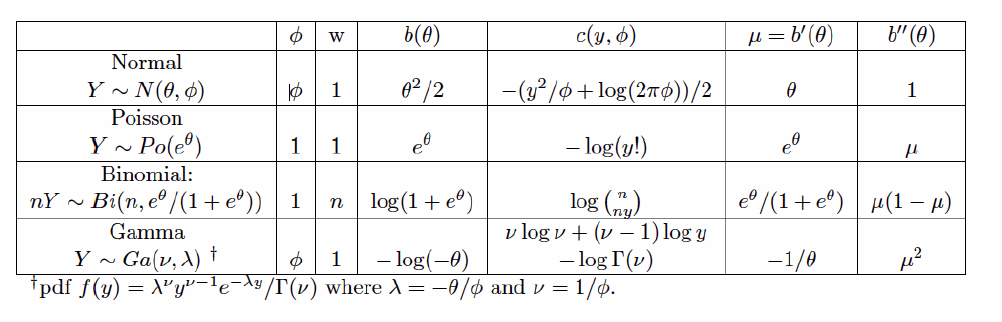
\includegraphics[width=0.7\linewidth]{glmdistribution}
	\end{center}
	
\end{document}